\documentclass{article}
\usepackage[12pt]{extsizes}
\usepackage[utf8]{inputenc}
\usepackage{amsmath}
\usepackage{amsfonts}
\usepackage{amssymb}
\usepackage{tabularx}
\usepackage{multirow}
\newcommand{\RomanNumeralCaps}[1]
{\MakeUppercase{\romannumeral #1}}
\usepackage{cmap} % для кодировки шрифтов в pdf
\usepackage[T2A]{fontenc}
\usepackage[russian]{babel}
\usepackage{graphicx} % для вставки картинок
\usepackage{amssymb,amsfonts,amsmath,amsthm} % математические дополнения от АМС
\usepackage{indentfirst} % отделять первую строку раздела абзацным отступом тоже
\usepackage[outdir=./]{epstopdf}
\usepackage{listings}
\usepackage{color} %red, green, blue, yellow, cyan, magenta, black, white
\definecolor{mygreen}{RGB}{28,172,0} % color values Red, Green, Blue
\definecolor{mylilas}{RGB}{170,55,241}
% Поля
\usepackage{geometry}
\geometry{left=2.5cm}
\geometry{right=1.5cm}
\geometry{top=1.5cm}
\geometry{bottom=2cm}

%%%%%%%%%%%%%%%%%%%%%%%%%%%%%%%    

\linespread{1.5} % полуторный интервал
\renewcommand{\rmdefault}{ftm} % Times New Roman
\frenchspacing

% подключаем hyperref (для ссылок внутри  pdf)
\usepackage[unicode, pdftex]{hyperref}

% коррекция подрисуночной подписи
\usepackage{caption}
\captionsetup[figure]{labelsep=period} %Точка
%\captionsetup[figure]{labelsep=space}  %Пробел
%\captionsetup[figure]{labelsep=endash}  %Новый страндарт
\usepackage[figurename=Рисунок]{caption}



\begin{document}
	
	\begin{titlepage}
		
		\begin{center}
			САНКТ-ПЕТЕРБУРГСКИЙ ГОСУДАРСТВЕННЫЙ ЭЛЕКТРОТЕХНИЧЕСКИЙ УНИВЕРСИТЕТ «ЛЭТИ» \\ИМ. В.И. УЛЬЯНОВА (ЛЕНИНА)\\
			\vspace{0.1cm}
			Кафедра Алгоритмической математики\\
			
			
			
		\end{center}
		
		\vspace{5cm}
		\begin{center}
			\begin{large}
				Лабораторная работа 2 \\
				"Алгоритм Ремеза"
			\end{large}
		\end{center}
		
		\vspace{5cm}
		
		\hspace{5cm} Студент гр.  0307 \hrulefill Латин Я.М.
		
		\vspace{0.5cm}
		\hspace{5cm} Преподаватель \hrulefill  Солнышкин С.Н.\\
		
		
		\vfill
		\begin{center}
			Санкт-Петербург\\
			2022
		\end{center}
		
		
	\end{titlepage}
	
	
	\newpage
	\tableofcontents
	\newpage
	\section{Цель работы}
	Построение многочлена наилучшего равномерного приближения с помощью алгоритма Ремеза.
	\section{Задание}
	С помощью алгоритма Ремеза найти многочлены наилучшего равномерного приближения 5-ой и 10-ой степени для функции $ f(x)=\dfrac{1000}{x^2-5x+60} $ на отрезке $[a;b]=[-1;7]$.\\
	
	\section{Построение многочленов}
	
		\subsection{Многочлен 5-ой степени}
		
		
			\subsubsection{Таблица результатов}
			\begin{flushright}
				Таблица 1. Результаты для многочлена 5 степени. 
			\end{flushright}
				
				\begin{table}[!h]
					\centering
					\begin{tabular}{|c|c|c|c|c|}
						\hline
						№ &\begin{tabular}[c]{@{}c@{}}уровень\\  квазиальтернанса\end{tabular} &
						
						\begin{tabular}[c]{@{}c@{}}глобальный  максимум \\погрешности\end{tabular} &
						\begin{tabular}[c]{@{}c@{}}точность\\  выравнивания\end{tabular} &
						\begin{tabular}[c]{@{}c@{}}номер точки, за \\ которой шёл максимум\end{tabular} \\ \hline
						1  & 0.0044918 & 0.017814   & 0.74785    & 1 \\ \hline
						2  & 0.0056883 & 0.015261   & 0.62726    & 6 \\ \hline
						3  & 0.0066137 & -0.012856  & 0.48556    & 2 \\ \hline
						4  & 0.0077863 & -0.010437  & 0.254      & 5 \\ \hline
						5  & 0.008251  & 0.0084858  & 0.027671   & 3 \\ \hline
						6  & 0.008294  & 0.008352   & 0.0069472  & 1 \\ \hline
						7  & 0.0083048 & 0.0083277  & 0.0027515  & 6 \\ \hline
						8  & 0.0083079 & -0.0083082 & 3.8933e-05 & 4 \\ \hline
						9  & 0.0083079 & -0.0083079 & 3.948e-13  & 2 \\ \hline
						10 & 0.0083079 & -0.0083079 & 3.948e-13  & 2 \\ \hline
					\end{tabular}
				\end{table}
			\newpage
			\subsubsection{Графики погрешностей}
				\begin{figure}[!h]
					\centering
				\begin{minipage}[!h]{0.47\linewidth}
					\center{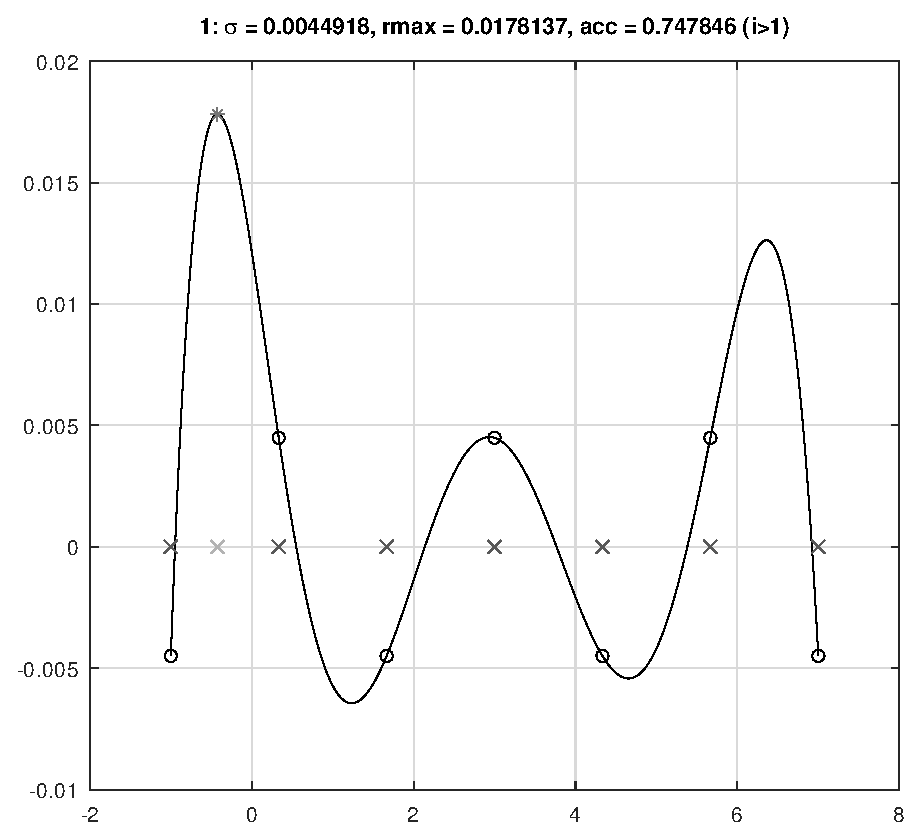
\includegraphics[width=1\linewidth]{../n5/1}}  \\
				\end{minipage}
				\hfill
				\begin{minipage}[!h]{0.47\linewidth}
					\center{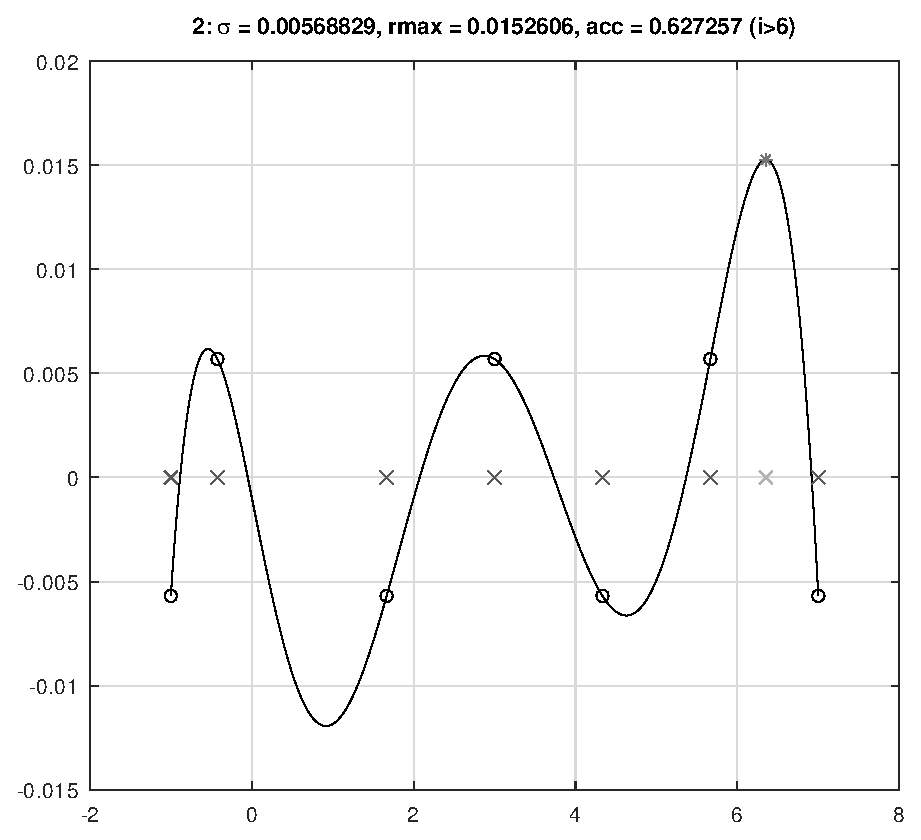
\includegraphics[width=1\linewidth]{../n5/2}} \\
				\end{minipage}
				\vfill
				\begin{minipage}[!h]{0.47\linewidth}
					\center{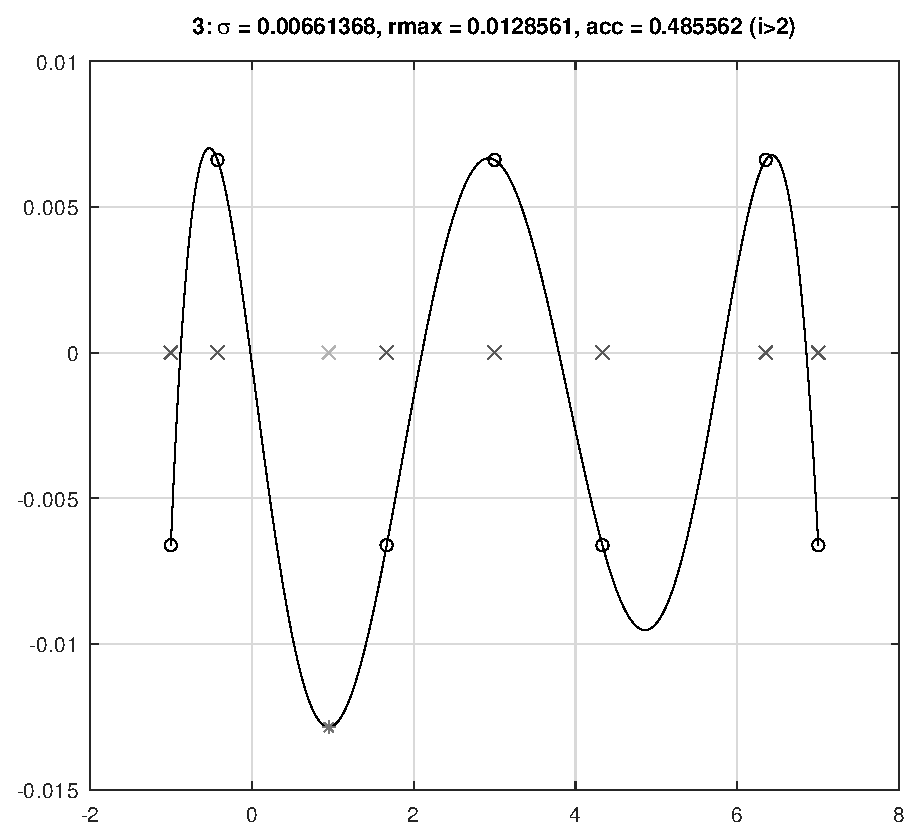
\includegraphics[width=1\linewidth]{../n5/3}}  \\
				\end{minipage}
				\hfill
				\begin{minipage}[!h]{0.47\linewidth}
					\center{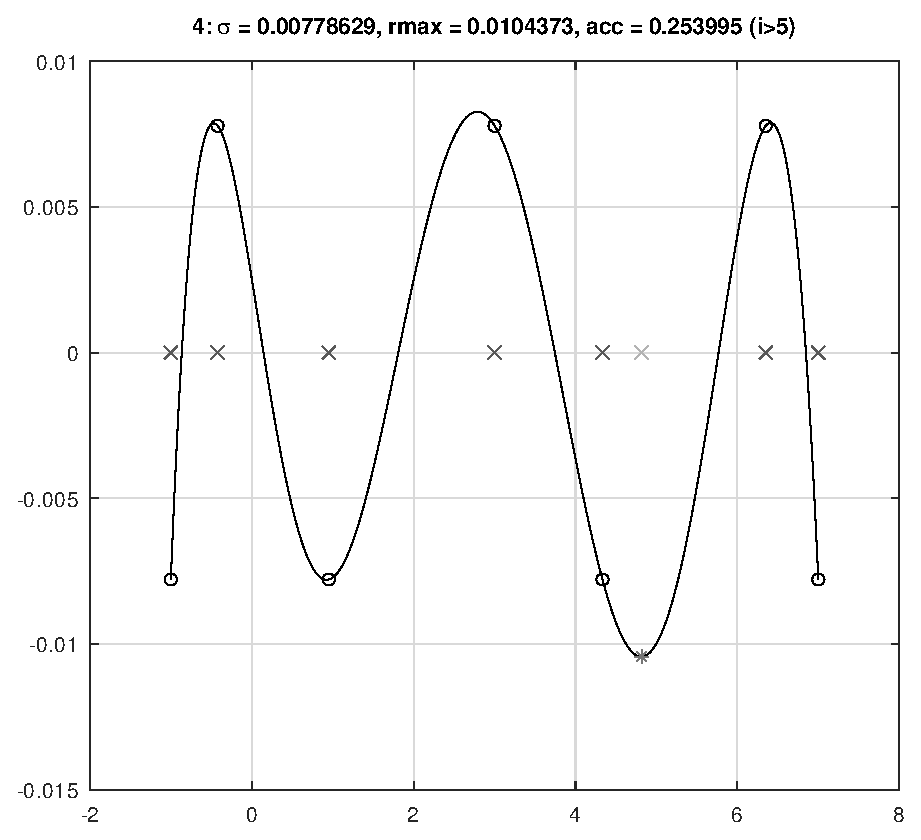
\includegraphics[width=1\linewidth]{../n5/4}}  \\
				\end{minipage}
				\vfill
				\begin{minipage}[!h]{0.47\linewidth}
					\center{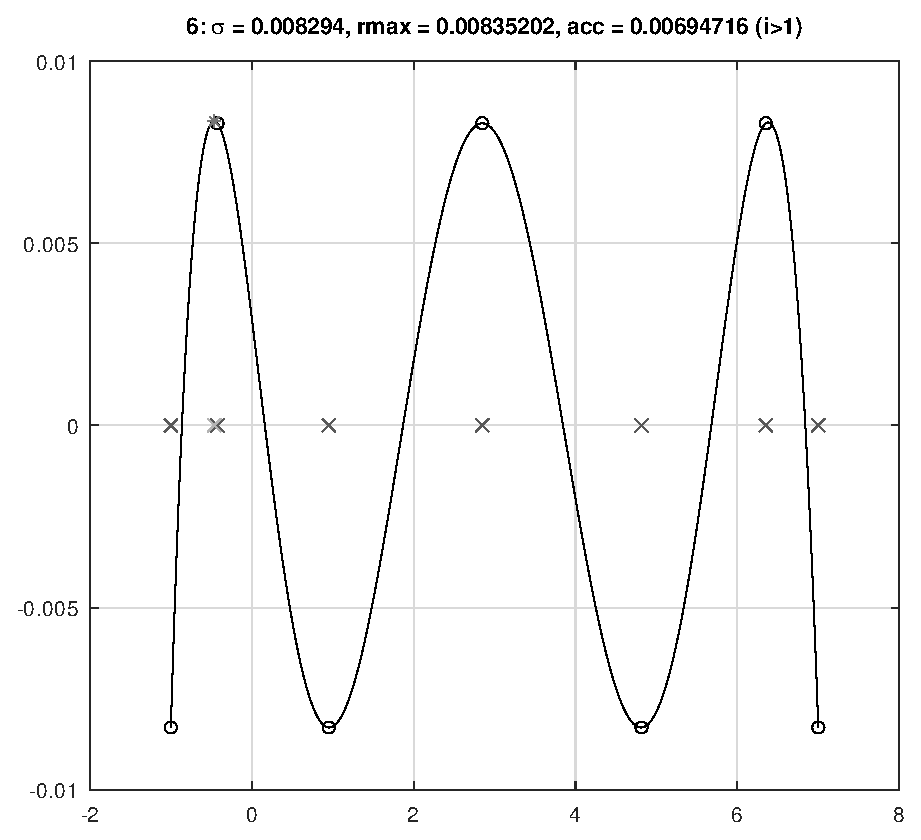
\includegraphics[width=1\linewidth]{../n5/6}}  \\
				\end{minipage}
				\hfill
				\begin{minipage}[!h]{0.47\linewidth}
					\center{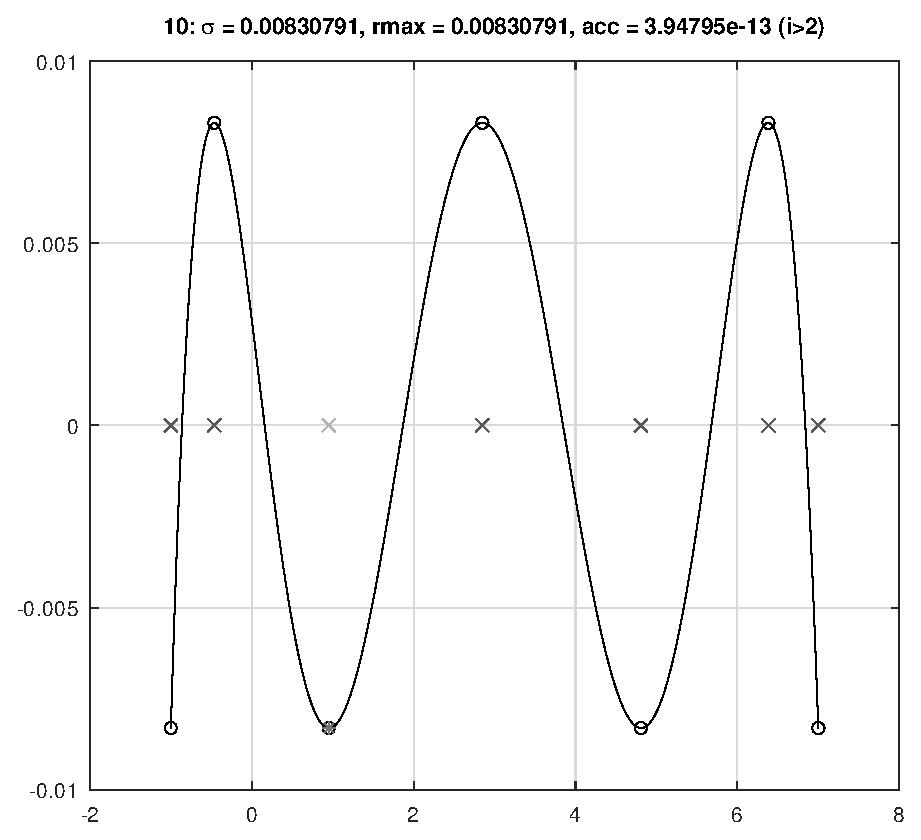
\includegraphics[width=1\linewidth]{../n5/10}} \\
				\end{minipage}
			\end{figure}
				\subsubsection{Найденный многочлен}
			$ L_5 =-0.0001740289x^5+0.0067366421x^4-
			0.0539489853x^3 $
			$ -0.1578708083x^2+1.4069231346x+16.6637573436 $
	\newpage
		\subsection{Многочлен 10-ой степени}
		
			
			\subsubsection{Таблица результатов}
			
				\begin{flushright}
					Таблица 2. Результаты для многочлена 10 степени.
				\end{flushright}
			
				\begin{table}[!h]
					\centering
					\begin{tabular}{|c|c|c|c|c|}
						\hline
						№ &\begin{tabular}[c]{@{}c@{}}уровень\\  квазиальтернанса\end{tabular} &
						
						\begin{tabular}[c]{@{}c@{}}глобальный максимум \\погрешности\end{tabular} &
						\begin{tabular}[c]{@{}c@{}}точность\\  выравнивания\end{tabular} &
						\begin{tabular}[c]{@{}c@{}}номер точки, за\\ которой шёл максимум\end{tabular} \\ \hline
						1  & 1.1532e-06 & -6.8242e-05 & 0.9831     & 11 \\ \hline
						2  & 1.3966e-06 & 4.4011e-05  & 0.96827    & 10 \\ \hline
						3  & 1.9122e-06 & 4.3149e-05  & 0.95568    & 1  \\ \hline
						4  & 2.1004e-06 & -2.7402e-05 & 0.92335    & 9  \\ \hline
						5  & 3.031e-06  & -3.4716e-05 & 0.91269    & 2  \\ \hline
						6  & 3.6141e-06 & 1.7896e-05  & 0.79805    & 3  \\ \hline
						7  & 4.3282e-06 & 1.8106e-05  & 0.76095    & 8  \\ \hline
						8  & 5.6253e-06 & -1.0224e-05 & 0.44977    & 4  \\ \hline
						9  & 6.0828e-06 & -9.3518e-06 & 0.34955    & 7  \\ \hline
						10 & 6.4682e-06 & -7.4483e-06 & 0.13159    & 11 \\ \hline
						11 & 4.1806e-06 & 7.1571e-05  & 0.94159    & 12 \\ \hline
						12 & 6.4682e-06 & -7.4483e-06 & 0.13159    & 11 \\ \hline
						13 & 6.556e-06  & 7.2279e-06  & 0.092958   & 10 \\ \hline
						14 & 6.6271e-06 & 7.0866e-06  & 0.06484    & 1  \\ \hline
						15 & 6.6482e-06 & -6.8099e-06 & 0.023758   & 9  \\ \hline
						16 & 6.6666e-06 & -6.7786e-06 & 0.016531   & 2  \\ \hline
						17 & 6.673e-06  & -6.6893e-06 & 0.0024452  & 5  \\ \hline
						18 & 6.6743e-06 & 6.6866e-06  & 0.0018417  & 5  \\ \hline
						19 & 6.6755e-06 & 6.684e-06   & 0.0012609  & 8  \\ \hline
						20 & 6.6765e-06 & -6.6778e-06 & 0.00019397 & 7  \\ \hline
						21 & 6.6766e-06 & -6.6766e-06 & 2.4617e-10 & 0  \\ \hline
						22 & 6.6766e-06 & -6.6766e-06 & 2.4617e-10 & 0  \\ \hline
					\end{tabular}
				\end{table}
			\newpage
			\subsubsection{Графики погрешностей}
			
			\begin{figure}[!h]
				\begin{minipage}[h]{0.47\linewidth}
					\center{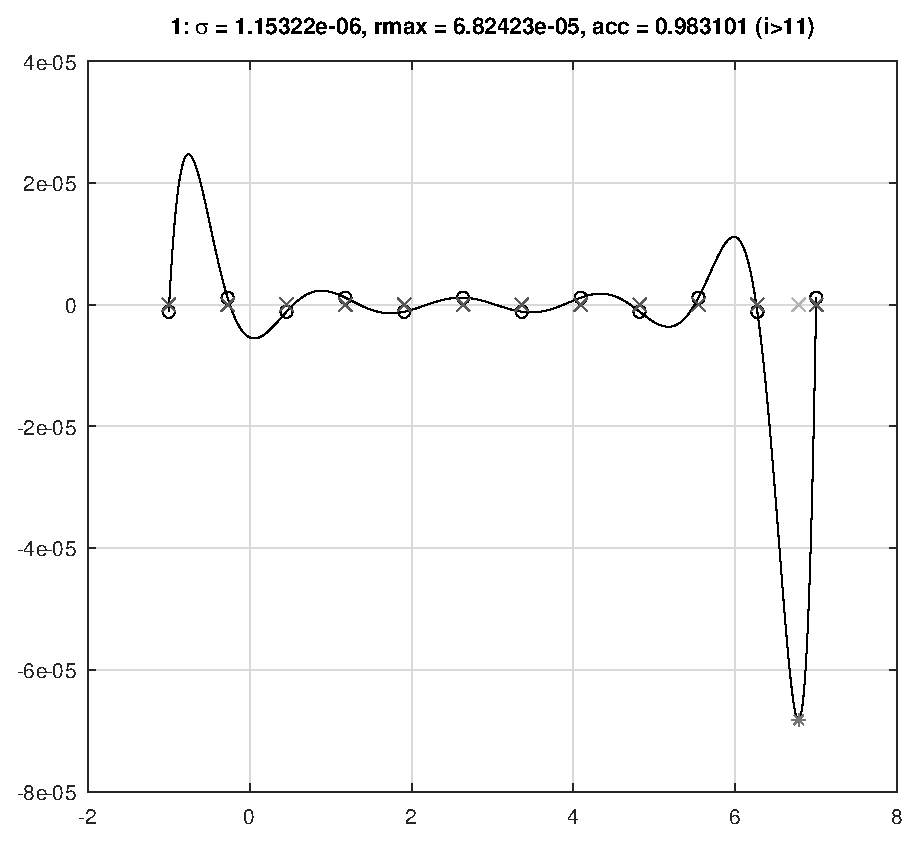
\includegraphics[width=1\linewidth]{../n10/1z}}  \\
				\end{minipage}
				\hfill
				\begin{minipage}[h]{0.47\linewidth}
					\center{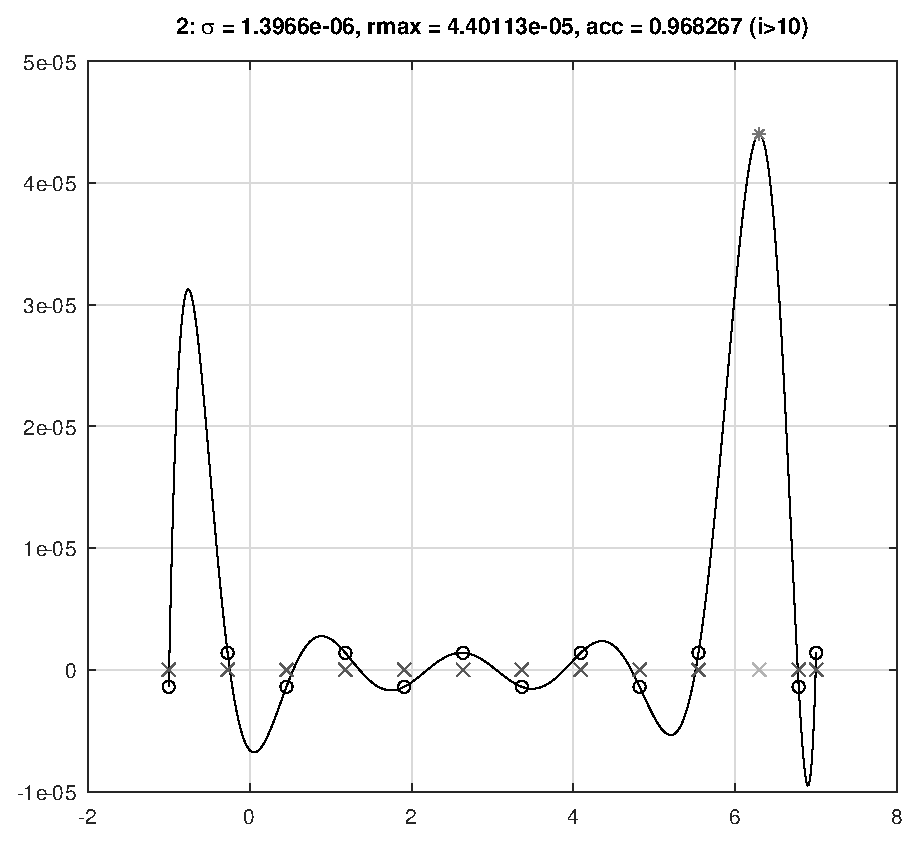
\includegraphics[width=1\linewidth]{../n10/2z}} \\
				\end{minipage}
				\vfill
				\begin{minipage}[h]{0.47\linewidth}
					\center{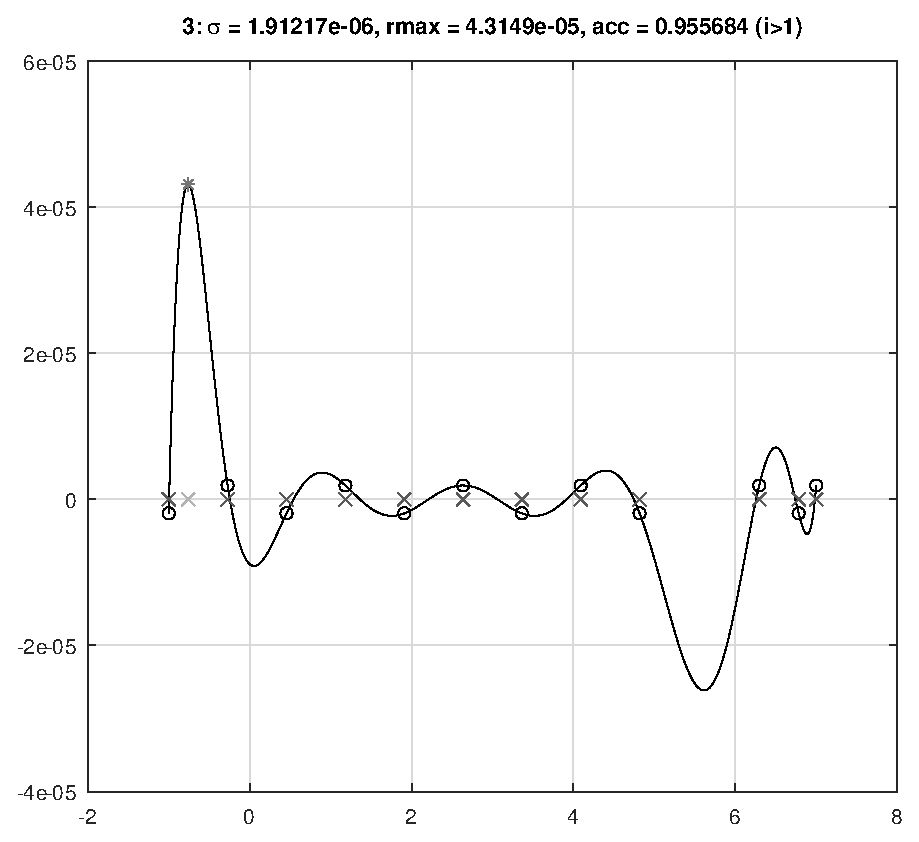
\includegraphics[width=1\linewidth]{../n10/3z}}  \\
				\end{minipage}
				\hfill
				\begin{minipage}[h]{0.47\linewidth}
					\center{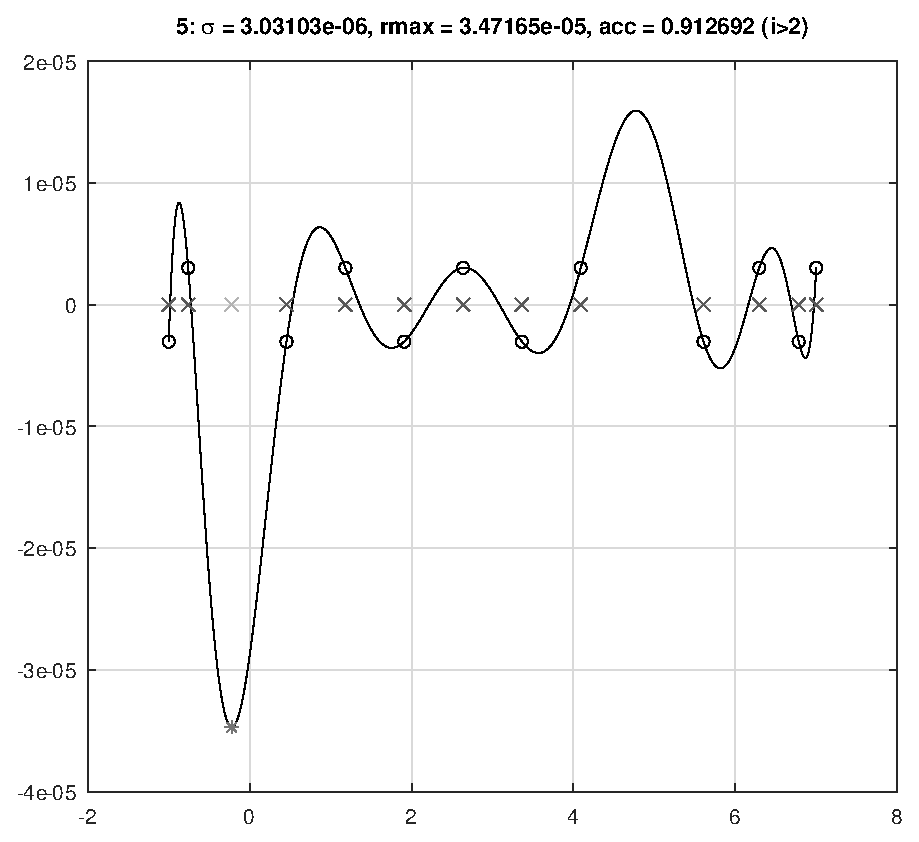
\includegraphics[width=1\linewidth]{../n10/5z}}  \\
				\end{minipage}
				\vfill
				\begin{minipage}[h]{0.47\linewidth}
					\center{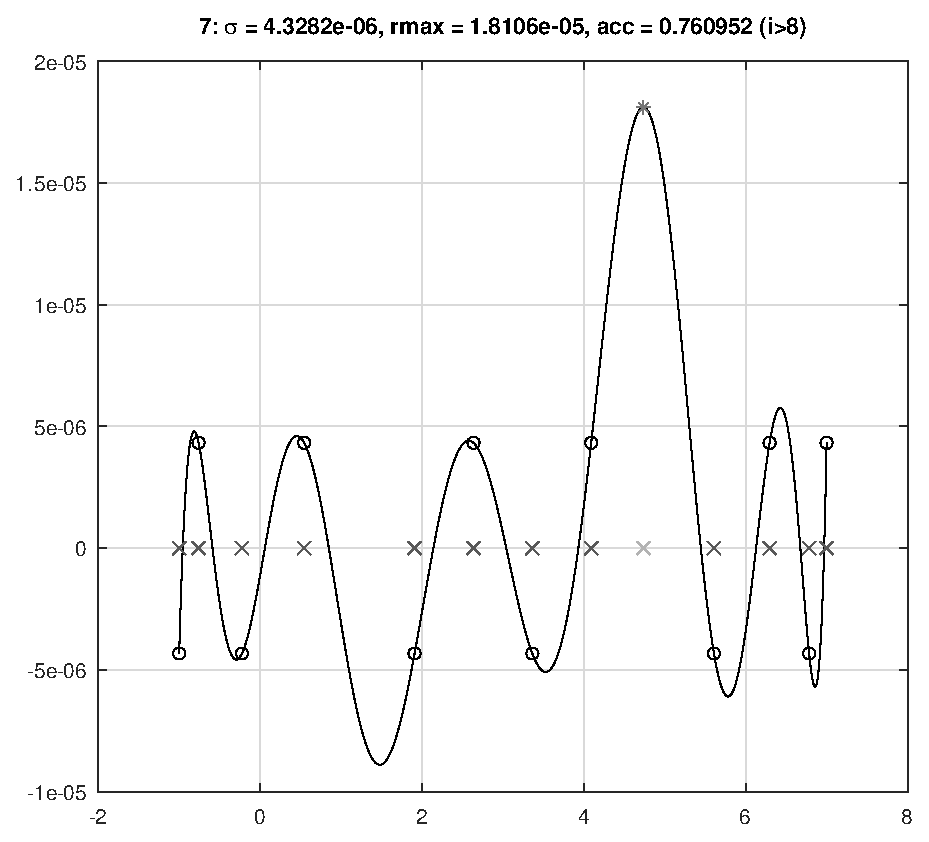
\includegraphics[width=1\linewidth]{../n10/7z}}  \\
				\end{minipage}
				\hfill
				\begin{minipage}[h]{0.47\linewidth}
					\center{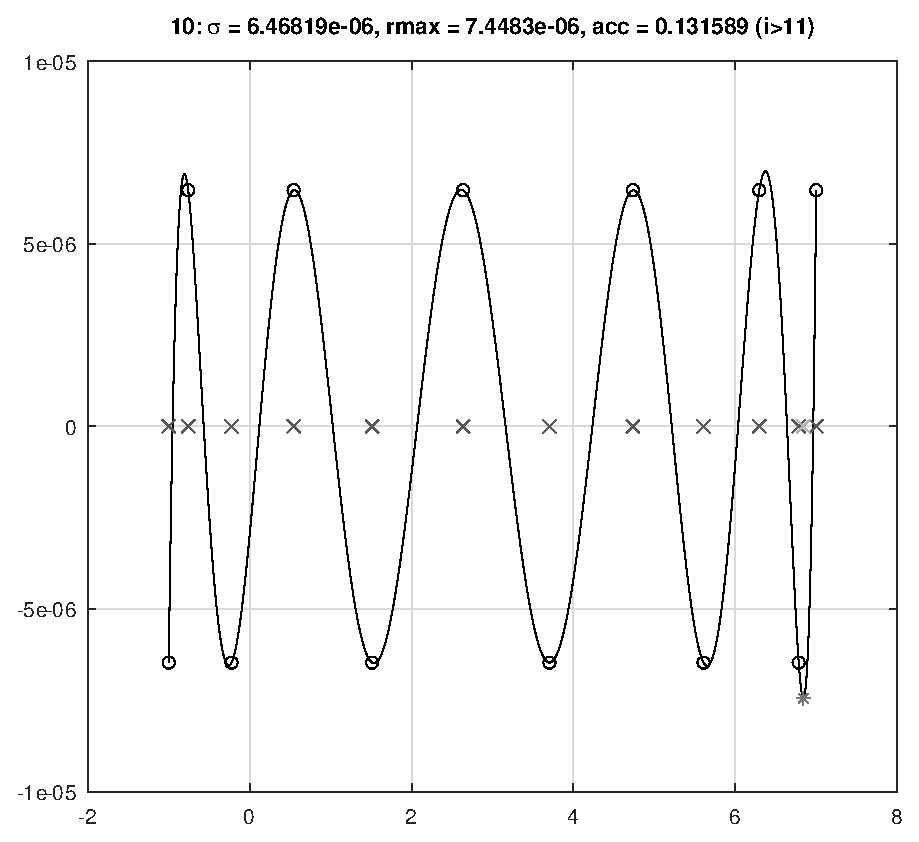
\includegraphics[width=1\linewidth]{../n10/10z}} \\
				\end{minipage}
			\end{figure}
		\newpage
			\begin{figure}[!h]
				
				\begin{minipage}[h]{0.47\linewidth}
					{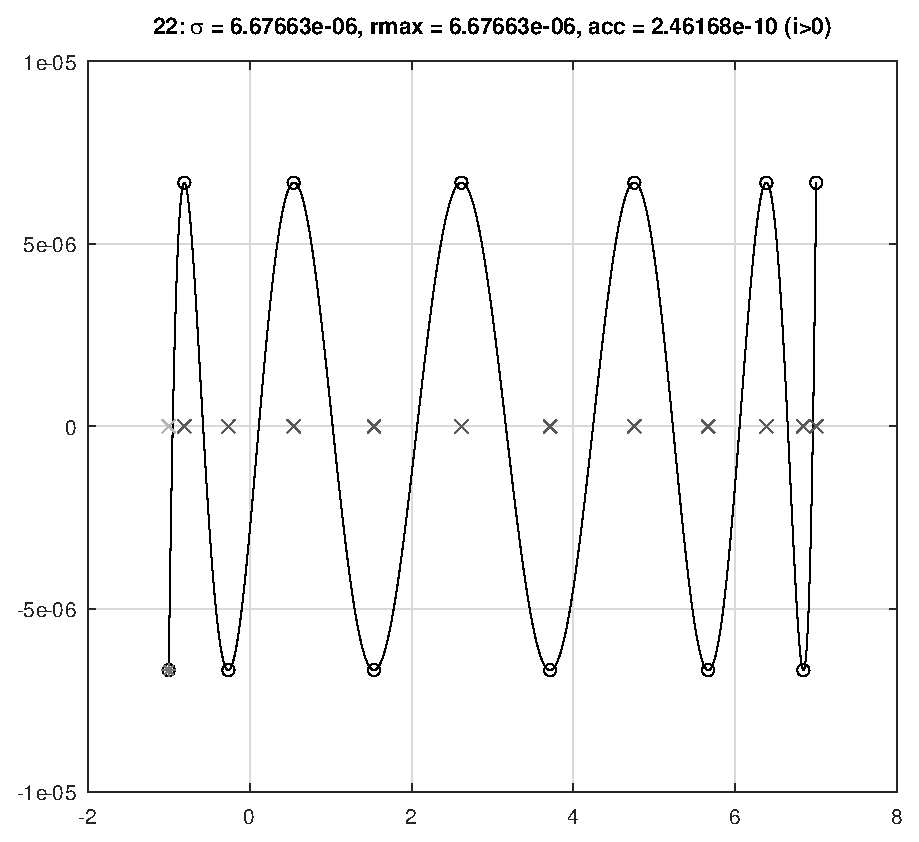
\includegraphics[width=1\linewidth]{../n10/22z}}  \\
				\end{minipage}
			\hfill
			\end{figure}

	\subsubsection{Найденный многочлен}
$L_{10} =
-1.3852195849\cdot 10^{-8}x^{10} +3.3481374149\cdot 10^{-7}x^9 -1.9035167286\cdot 10^{-6}x^8
-1.0988223274\cdot 10^{-5}x^7 + 8.4121387845\cdot 10^{-5}x^6 + 0.0005363647x^5
-0.0003641573x^4 - 0.0365801852x^3 - 0.1620555088x^2 +
1.3888647251x + 16.6666695414$

\lstset{language=Matlab,%
	%basicstyle=\color{red},
	breaklines=true,%
	morekeywords={matlab2tikz},
	keywordstyle=\color{blue},%
	morekeywords=[2]{1}, keywordstyle=[2]{\color{black}},
	identifierstyle=\color{black},%
	stringstyle=\color{mylilas},
	commentstyle=\color{mygreen},%
	showstringspaces=false,%without this there will be a symbol in the places where there is a space
	numbers=left,%
	numberstyle={\small \color{black}},% size of the numbers
	numbersep=9pt, % this defines how far the numbers are from the text
	emph=[1]{for,end,break},emphstyle=[1]\color{red}, %some words to emphasise
	%emph=[2]{word1,word2}, emphstyle=[2]{style},    
}
	\newpage
	\section{Код сценариев и функции}
	\section*{W05.m}
	\lstinputlisting{../w05.m}
	\section*{W010.m}
	\lstinputlisting{../w010.m}
	\newpage
	\section*{W1.m}
	\lstinputlisting{../w1.m}
	\newpage
	\section*{sys.m}
	\lstinputlisting{../sys.m}
	\section*{f.m}
	\lstinputlisting{../f.m}
	\end{document}